\documentclass[tikz,border=1pt]{standalone} 
\usepackage{tikz}
% \usepackage{automata, arrows}
\usetikzlibrary{arrows.meta,calc,decorations.markings,math,arrows.meta}
\usetikzlibrary{positioning}
\begin{document}
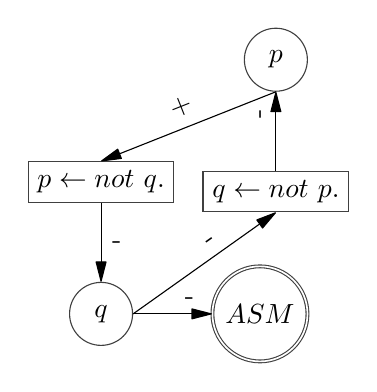
\begin{tikzpicture} [
    atom/.style={circle,  draw=black!75, minimum size=8mm},
    rule/.style={rectangle, draw=black!75, minimum size=3mm},
    sink/.style={circle, double, draw=black!75, minimum size=3mm},
    dummy/.style={midway,sloped,left,rotate=270},
    dummy2/.style={midway,sloped,left},
    >={Stealth[inset=0pt,length=8pt,angle'=28,round]}
    ]
    %Nodes
    \node[atom]      (p)       {$p$};
    \node[rule]      (rpnotq)       [below left=of p] {$p \leftarrow not\ q.$};
    \node[atom]      (q)      [below =of rpnotq] {$q$};
    \node[rule]      (rqnotp)  [below =of p] {$q \leftarrow not\ p.$};
    \node[sink]      (asm)  [right =of q] {$ASM$};

    %Lines
    \draw[->] (p.south) -- (rpnotq.north) node[dummy] {+};
    \draw[->] (rpnotq.south) -- (q.north) node[dummy] {-};
    \draw[->] (q.east) -- (rqnotp.south) node[dummy2, yshift=0.2cm, xshift=0.4cm] {-};
    \draw[->] (rqnotp.north) -- (p.south) node[dummy2, yshift=0.2cm, xshift=0.4cm] {-};
    \draw[->] (q.east) -- (asm.west) node[dummy2, yshift=0.2cm, xshift=0.4cm] {-};

\end{tikzpicture} 
\end{document}